Since the First Year Report, in which I attempted to go straight for a continuum-limit model and was largely unsuccessful, I have decided to change my approach to the problem a bit.
I attended a conference on Diffusion in Dresden last September, and there I spoke with people from many different disciplines. The general feeling was that a computational lattice-based approach
would be a good starting point, as this would allow me to perform calculations which I could then use to derive continuum-limit PDEs, as well as providing potentially useful information about the Titanium
Dioxide/Titanium interface and its dynamics. In the following subsections, I will give a summary of my activities since last September.

\subsection{Finding a Computational Framework}

In order to perform Monte-Carlo lattice dynamics calculations, I could have written my own code from scratch. However, if I were to have done do that, I would have spent a lot of time working out how to implement
Gillespie-like algorithms, then would have had to write and debug code and a whole host of other time-consuming things. Instead, I looked for pre-existing software packages which fulfilled my requirements.

Of those I looked into, \texttt{KMCLib}\cite{leetmaa2014kmclib} looked to be the most suited to my requirements. It uses Python for configuring the calculations, and then performs them using C++ for speed
and, if desired, parallelisation. I have now spent a while using this code, and after some teething problems am satisfied that it can do what I need it to do and that I can use it correctly.

\subsection{Choice of Model}
\label{sec: modelChoice}

So, it is all very well to say that we wish to model the diffusion of Oxygen through a Titanium lattice using stochastic lattice dynamics, but what kind of model should we use? I decided to work in
one-dimensional systems instead of three-dimensional systems to begin with. This is because:
\begin{itemize}
 \item As Titanium corrodes, the oxide layer advances forward as a broad front; therefore the problem is essentially one-dimensional;
 \item There aren't nearly so many one-dimensional models as there are three-dimensional models; thus a one-dimensional model should have fewer free parameters, and therefore stronger predictive power;
 \item We can perform calculations much faster in one-dimensional models than in three-dimensional models, so if our one-dimensional model is terrible, we should find out fairly quickly!
\end{itemize}
Thus, I am in the processing of investigating the phenomenology of the following lattice model, which is about the simplest one can make which should produce the behaviour we're looking for:
\begin{itemize}
 \item Let there be a one-dimensional chain of $L$ lattice sites. Each site is occupied by either an Oxygen atom (denoted by $O$) or a Vacancy (denoted by $V$). For example, a particular
 chain of length 5 could be configured $OOVOV$.
 \item In a stochastic model, we randomly transition to new configurations with certain rates. In our model we would like Oxygen atoms to be able to hop into vacant spaces, imitating how Oxygen atoms move
 between interstitial voids in Titanium. Clearly then, we only wish to allow
 transitions in which adjacent Oxygens and Vacancies swap places. 
 \item The rates for my model are as follows:
 \begin{center}
  \begin{tabular}{c c c c}
  $\cdots VOVV\cdots$ & $\longrightarrow$ & $\cdots VVOV \cdots$ & with rate $1$ \\
  $\cdots VOVO\cdots$ & $\longrightarrow$ & $\cdots VVOO \cdots$ & with rate $1$ \\
  $\cdots OOVV\cdots$ & $\longrightarrow$ & $\cdots OVOV \cdots$ & with rate $\lambda$ \\
  $\cdots OOVO\cdots$ & $\longrightarrow$ & $\cdots OVOO \cdots$ & with rate $\lambda$, \\
 \end{tabular}
 \end{center}
 as well as the 4 counterpart transitions and rates one finds by requiring left-right mirror symmetry. More simply, an Oxygen can jump forward into an empty Vacancy with rate $1$ if there is a Vacancy behind its starting
 position, and with rate $\lambda$ if the position behind it contains and Oxygen. This is supposed to indicate short-range attraction ($\lambda < 1$) or repulsion ($\lambda > 1$) between Oxygen atoms.

\end{itemize}

I intend to use the model outlined above with $\lambda<1$, so that Oxygen atoms are attracted to one another. It may not be obvious, but one can show that the above model does obey the Principle of Detailed Balance, with an ``energy''
proportional to the number of Oxygen-Oxygen adjacencies (one might think of these as ``Oxygen bonds'').

\subsection{Model Predictions}
\begin{figure}[h!]
\centering
 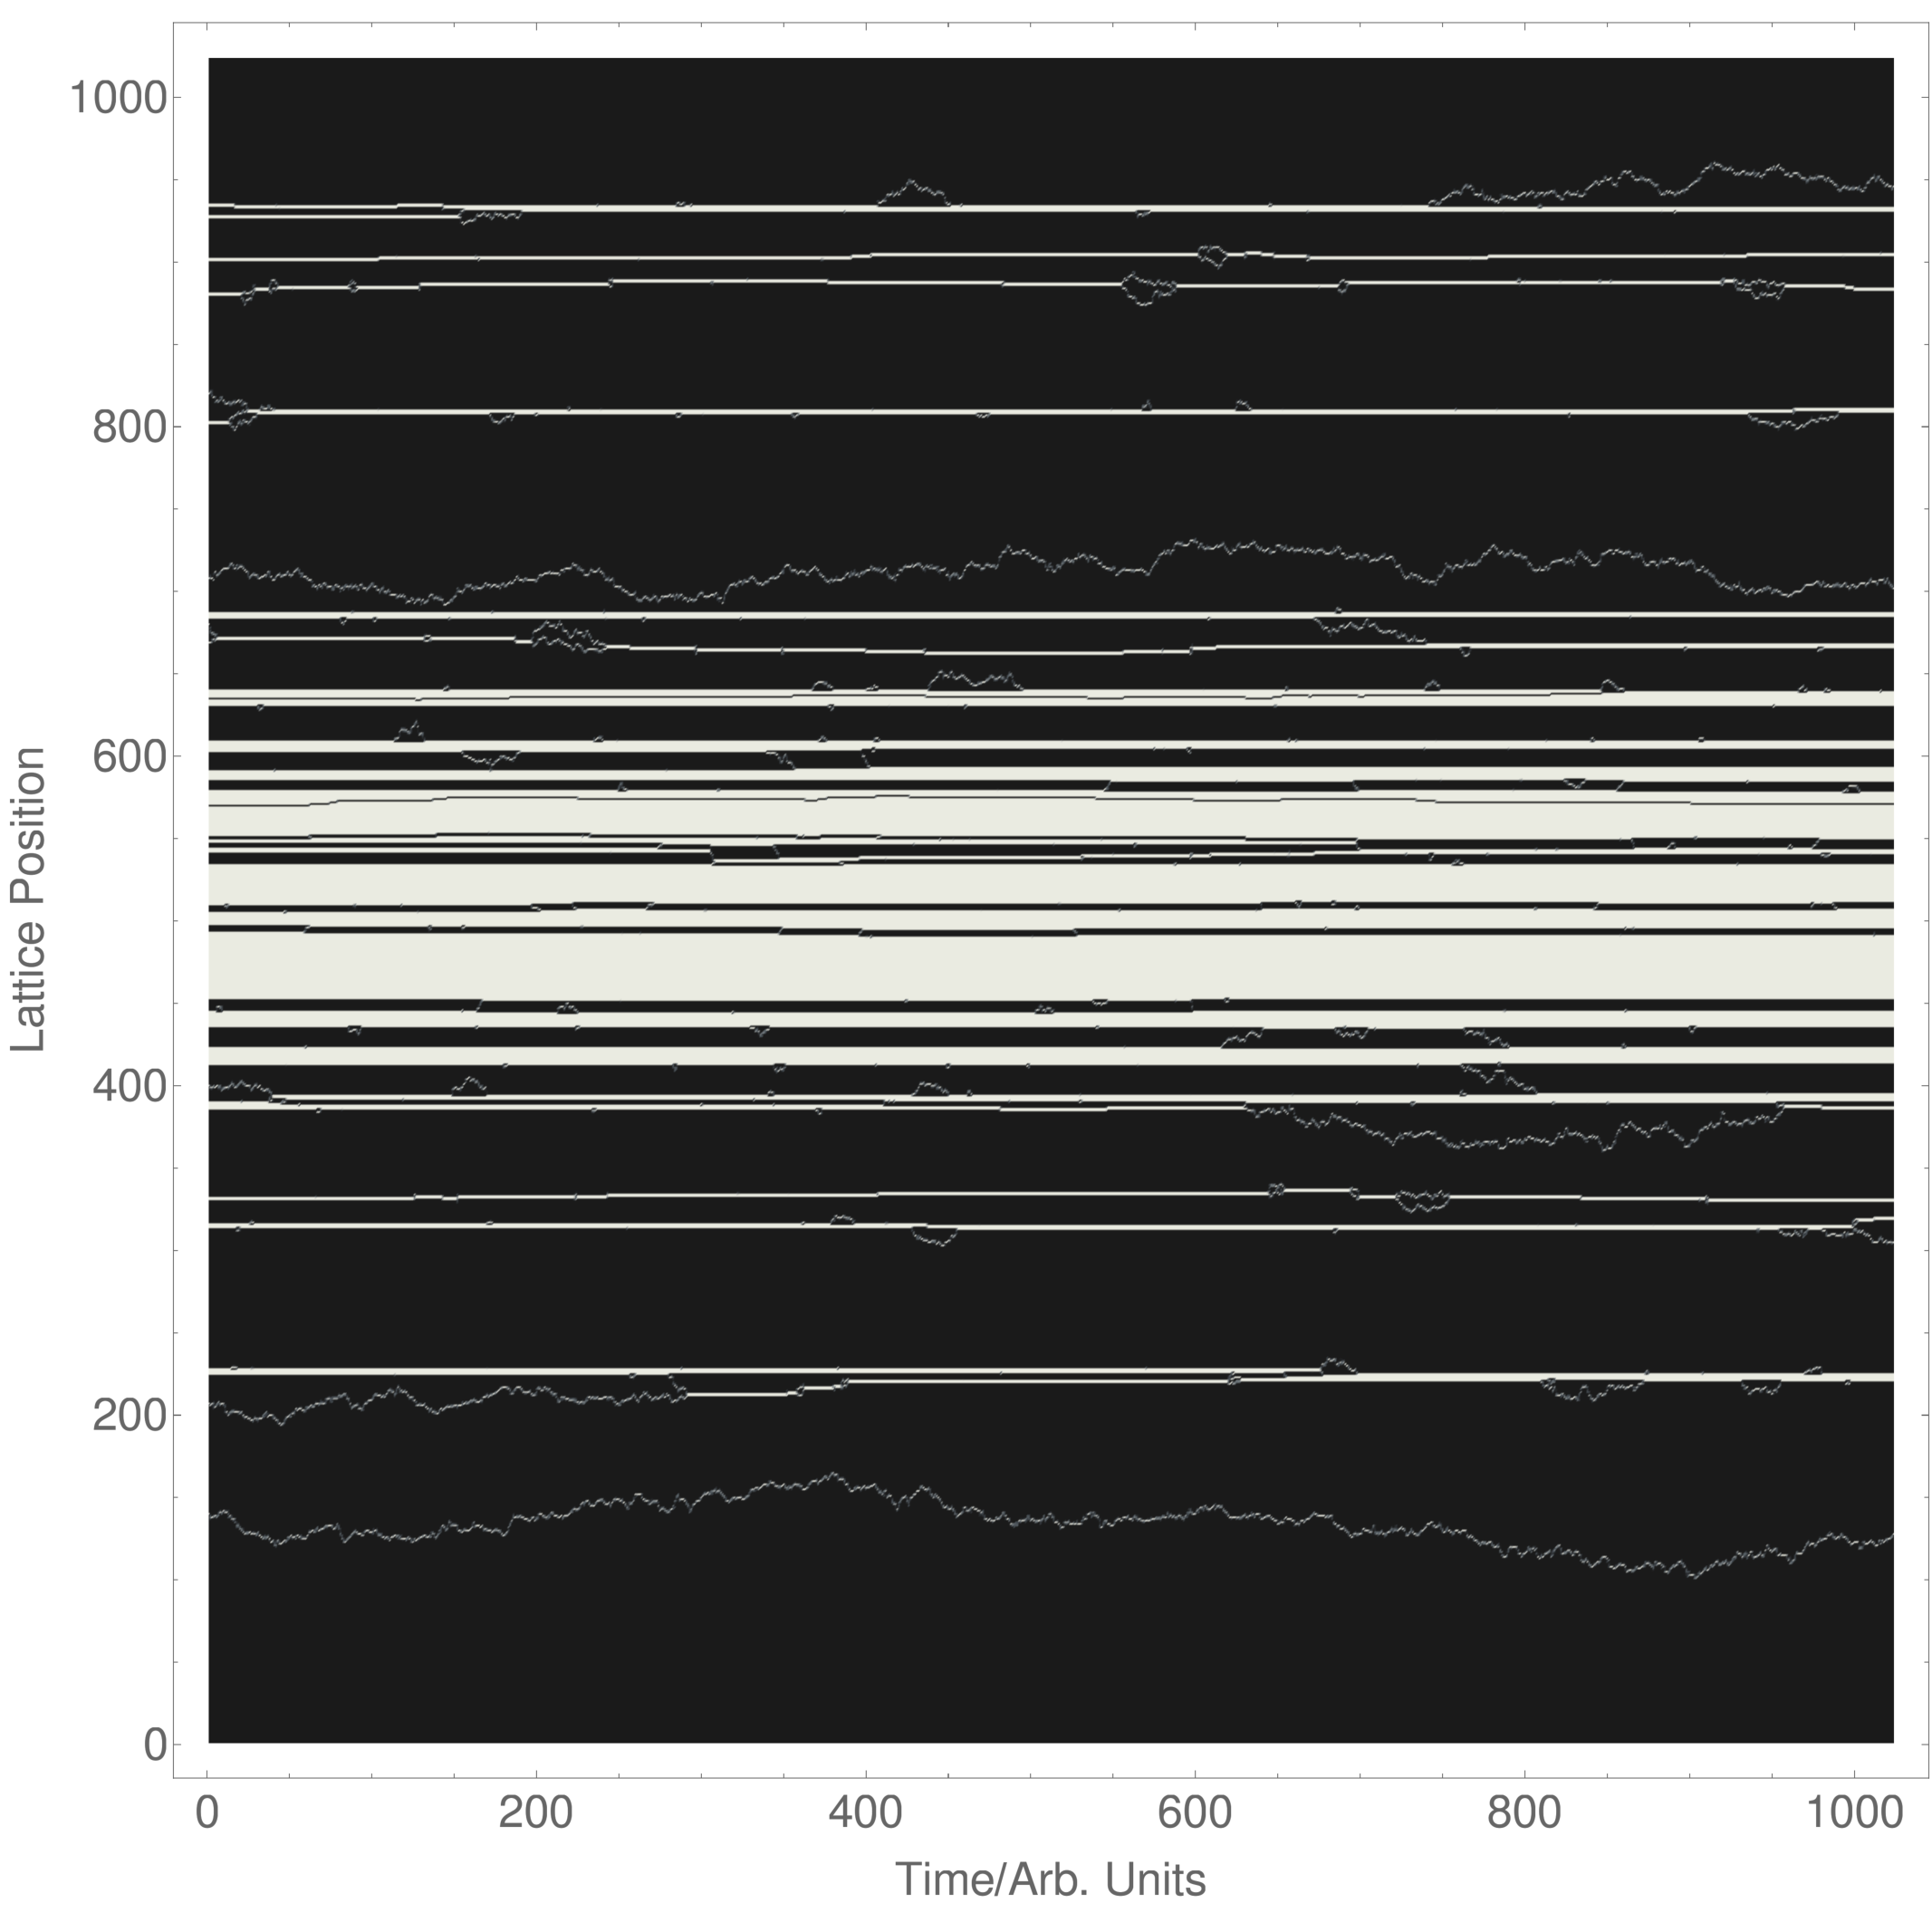
\includegraphics[width=\textwidth]{../tex-src/images/periodicExample}
 \caption{The time-evolution of a closed periodic system (size 1024) containing a fixed number of O and V. Each pixel is shaded according to the time-averaged occupation of that particular site during that time period (in other words,
 if we let the occupation be 1 if there is an O there and 0 for a V, what is the average of this occupation over a short time interval?):
 white indicates high average occupation, around 0; black indicates low occupation. In this case, $\lambda=0.01$. Notice the solid blocks of Oxygen-rich material more than two Oxygens thick, often surrounded by a halo of sparse gassy individual Oxygens undergoing random walks.}
 \label{fig: periodicExample}
\end{figure}

\begin{figure}[h]
\centering
 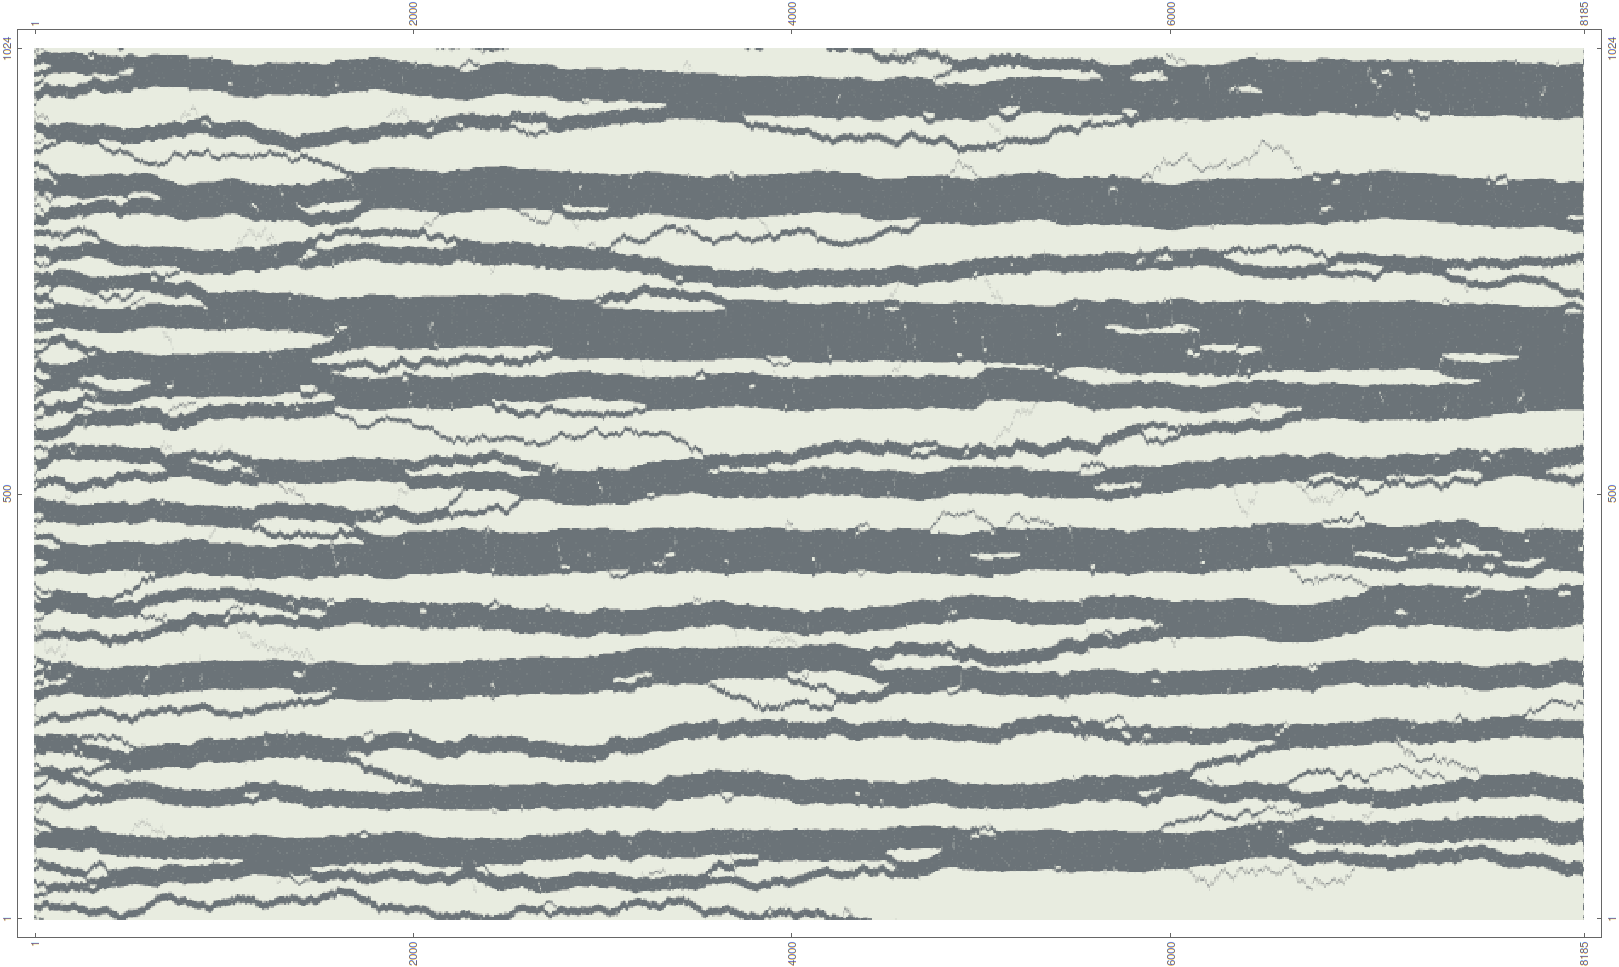
\includegraphics[width=\textwidth]{../tex-src/images/fractures1}
 \caption{A plot done using the same technique as Figure~\ref{fig: periodicExample}, again with periodic boundary conditions. This computation was performed with a similar value of $\lambda$ but over a much longer time period.
 In this case, the initial configuration had a random 50:50 mix of O and V. Notice how the Vacancy-rich
 regions form streams which walk randomly whilst retaining roughly the same width, occasionally coalescing and splitting.}
 \label{fig: fractureExample}
\end{figure}
     
I originally intended to quickly investigate the way the Oxygen flows through a one-dimensional chain, by imposing boundary conditions equivalent to different concentrations at different ends of the chain and measuring how rapidly
the Oxygen flows with different concentration gradients and in different average-concentration environments. However, it then occurred to me that this system might exhibit some phase equilibrium phenomena, which would be best investigated
by considering the problem to have periodic boundary conditions and simply setting up a mixtures of Oxygen and Vacancies and then seeing how they behave for a given value of $\lambda$. In order to check that the simulations are proceeding
as desired, I have put some effort into being able to record and view the system's behaviour over time; a visualisation of an example system's time evolution is displayed in Figure~\ref{fig: periodicExample}.
As of writing this paper, this numerical work is still ongoing; the code needs to be refactored a little before it is ready for bulk use.

We can also make progress using analytics. So far, I have managed to derive the mean-field theory, with a little help from Martin Evans. If $\rho_i (t)$ is the mean-field average occupation of the $i^\mathrm{th}$ site at time $t$, then
it should obey
\begin{equation}
 \partDeriv{\rho_i}{t} = \left( 1-\rho_i \right) \left[ \left(1-\zeta\rho_{i-2} \right) \rho_{i-1} + \left(1-\zeta\rho_{i+2} \right) \rho_{i+1} \right]
 - \rho_i \left[ 2 \zeta \rho_{i-1} \rho_{i+1}  - (3-\zeta)\left(\rho_{i-1} + \rho_{i+1}\right) + 2 \right],
\end{equation}
where $\zeta = 1-\lambda$ seems to be the most appropriate way to express the degree of nonlinearity in the system. If we let the spacing between the lattice sites be $a$, and promote $\rho_i (t)$ to $\rho(x, t)$, a continuous
spacetime variable, then we find that in the long-wavelength limit it should obey
\begin{equation}
 \partDeriv{\rho}{t} = \frac{1}{2} a^2 \left[ \left( 2 - 2 \zeta \rho (4-3\rho) \right) \partDeriv{^2 \rho}{x^2} - \zeta \left(2-3\rho\right) \left(\partDeriv{\rho}{x}\right)^2 \right] + \mathcal{O}(a^4).
 \label{eq: longRangePDE}
\end{equation}
Later on, I would like to use these PDEs to help simulate large-scale aspects of the Titanium/Titanium Dioxide problem.

Finally, it possible to make limited predictions about equilibrium. As I have stated, the number of Oxygen-Oxygen ``bonds'' makes a god candidate for the energy of the system. Thus, we may be able to use this to tell if phase separation has
occurred or not. By making a few simplifying assumptions, one can show that for a closed sample with Oxygen number density $\rho_0$, the average number of bonds per Oxygen is 
\begin{equation}
 1 + \frac{\lambda \left( \rho_0 -1 \right)}{\rho_0},
 \label{eq: eqmBehaviour}
\end{equation}
so long as $\lambda < \rho$. Exploring the validity of this theory is one of the immediate goals of my current numeric work.



